\documentclass[conference]{IEEEtran}
\IEEEoverridecommandlockouts

\usepackage{cite}
\usepackage{amsmath,amssymb,amsfonts}
\usepackage{algorithmic}
\usepackage{graphicx}
\usepackage{textcomp}
\usepackage{xcolor}
\usepackage{booktabs}
\usepackage{array}
\usepackage{tikz}
\usetikzlibrary{shapes.geometric, arrows.meta, positioning}
\usepackage[hidelinks]{hyperref}

\graphicspath{{figures/}}

\def\BibTeX{{\rm B\kern-.05em{\sc i\kern-.025em b}\kern-.08em T\kern-.1667em\lower.7ex\hbox{E}\kern-.125emX}}

\begin{document}

\title{Explainable Hybrid Machine Learning for Multi-Class Disease
Classification: A Study of Anemia CBC Data and Large-Scale\\
Thyroid Diagnosis}

\author{
\IEEEauthorblockN{Aditya Dhull}
\IEEEauthorblockA{\textit{Independent Study in Applied Machine Learning} \\
\texttt{adityadhull@iisc.ac.in}}
}

\maketitle

\begin{abstract}
Automated classification of hematologic and endocrine disorders from routine
laboratory panels can assist clinical decision support, but reported systems
often rely on small single-source datasets, neglect class imbalance and missing
values, and provide only global explanations. This paper presents a unified,
reproducible, and explainable framework and evaluates it in two experiments.
\emph{Experiment~1} applies a hybrid Random~Forest (RF) and Extreme
Gradient Boosting (XGBoost) soft-voting framework to nine-class anemia
classification from Complete Blood Count (CBC) data ($n{=}1{,}232$ after
de-duplication). \emph{Experiment~2} extends the same pipeline to a substantially
larger and harder problem: seven-class thyroid-disease diagnosis from the Garavan
Institute archive ($n{=}9{,}172$), which contains severe class imbalance
($73.8\%$ majority) and informative missing laboratory values. The framework adds
stratified five-fold cross-validation, macro-averaged metrics, one-vs-rest
ROC--AUC, paired significance testing, and---crucially---\emph{detailed
per-prediction} SHapley Additive exPlanations (SHAP). On anemia the hybrid
attains a hold-out accuracy of $0.984$ and macro-F1 of $0.947$. On thyroid it
attains accuracy $0.945$ and macro-F1 $0.863$. We find that the hybrid's
improvement over the RF baseline is \emph{not} statistically significant on
anemia ($p{=}0.82$),
and we further show, via a seed-stability analysis, that a five-fold paired
$t$-test p-value is itself unstable (range $0.03$--$0.99$); on the $7\times$
larger thyroid data the analogous improvement \emph{is} significant ($p{=}0.014$),
illustrating that statistical power---not a better model---drives the difference.
SHAP explanations align with established physiology and, in one case, expose a
data-quality error, demonstrating the practical value of instance-level
interpretability.
\end{abstract}

\begin{IEEEkeywords}
Anemia, thyroid disease, XGBoost, Random Forest, soft voting, SHAP, explainable
AI, class imbalance, macro-F1, statistical significance.
\end{IEEEkeywords}

\section{Introduction}
Routine laboratory panels such as the Complete Blood Count (CBC) and the thyroid
function panel are inexpensive, ubiquitous, and information-rich. Machine learning
(ML) over such structured data can support the differential diagnosis of disorders
whose subtypes carry distinct clinical management. However, three recurring
weaknesses limit the trustworthiness of reported systems: (i) reliance on small,
single-institution datasets; (ii) inadequate treatment of class imbalance and
missing values; and (iii) explanations restricted to global feature importance,
without per-patient justification.

This work is organized around a single, leakage-safe pipeline applied to two
diseases. We first \emph{apply} a hybrid RF\,$+$\,XGBoost soft-voting framework
to nine-class anemia classification, with a leakage-safe preprocessing,
evaluation protocol, and SHAP-based interpretation. We then \emph{extend} the
identical pipeline to a larger, more complex thyroid-disease problem deliberately
chosen to stress the three weaknesses above. Our contributions are:
\begin{itemize}
\item A careful, open anemia classification study reporting an \emph{honest}
negative result on statistical significance.
\item An extension to seven-class thyroid diagnosis on $9{,}172$ patients with
explicit handling of severe imbalance and informative missingness.
\item Detailed \emph{per-prediction} SHAP narratives that decompose individual
predictions into clinically interpretable contributions, including for
mis-classified cases.
\item A seed-stability analysis showing that a five-fold paired $t$-test p-value
is intrinsically noisy, and a demonstration that the hybrid's advantage becomes
statistically detectable only with a larger sample.
\end{itemize}

\section{Related Work}
Classical anemia classification follows morphological reasoning on the mean
corpuscular volume (MCV) and the hemoglobin (HGB) concentration, distinguishing
microcytic, normocytic, and macrocytic anemias, refined by MCH and MCHC. Recent
ML studies report high accuracy with tree ensembles on CBC data, and growing use
of SHAP for interpretability. The hybrid framework studied here couples RF
and XGBoost via soft voting, applies SHAP to the boosted component, and---unlike
much prior work---tests whether the hybrid's gain over a baseline is statistically
significant.

Thyroid-disease classification from the Garavan archive is a long-standing
benchmark. Its laboratory features (TSH, T3, TT4, T4U, FTI) map directly to the
hypothalamic--pituitary--thyroid feedback loop, making it an ideal substrate for
verifying that learned attributions match physiology. Its size, imbalance, and
structured missingness make it markedly more challenging than the anemia panel,
which is precisely why we adopt it for the extension.

\section{Datasets}
Table~\ref{tab:data} summarizes both datasets. The anemia CBC dataset comprises
14 numeric features and nine diagnostic classes; we remove exact duplicate
records (a standard de-duplication step) leaving $1{,}232$ patients.
The thyroid dataset (\texttt{thyroid0387}) comprises $9{,}172$ records; we map the
raw diagnosis codes into seven clinically coherent groups (negative, hypothyroid,
hyperthyroid, binding-protein anomaly, non-thyroidal illness, replacement therapy,
discordant results). Thyroid features mix six continuous laboratory values, 14
binary clinical-history flags, and two nominal categoricals, and contain
substantial missingness (e.g.\ T3 missing in $28\%$ of records). Crucially, this
missingness is \emph{informative}---a test is ordered when clinically
suspected---so we retain it via missing-indicator features rather than discarding
it.

\begin{table}[t]
\caption{Dataset characteristics.}
\label{tab:data}
\centering
\renewcommand{\arraystretch}{1.2}
\begin{tabular}{lcc}
\toprule
& \textbf{Anemia (CBC)} & \textbf{Thyroid (Garavan)} \\
\midrule
Patients & 1{,}232 & 9{,}172 \\
Classes & 9 & 7 \\
Features & 14 numeric & 6 lab $+$ 14 binary $+$ 2 nominal \\
Majority class & 26.2\% & 73.8\% \\
Missing values & none & yes (informative) \\
\bottomrule
\end{tabular}
\end{table}

\section{Methodology}
\subsection{Preprocessing}
Let the dataset be $D=\{(x_i,y_i)\}_{i=1}^{N}$ with $x_i\in\mathbb{R}^d$ and
$y_i\in\{1,\dots,K\}$. Numeric features are median-imputed with an appended binary
missing-indicator; nominal features are most-frequent imputed and one-hot
encoded. Because tree ensembles are invariant to monotone feature scaling, no
standardization is applied. All transformers are fit \emph{inside} the
cross-validation loop so that no validation-fold statistics leak into training.

\subsection{Hybrid Ensemble and Extensions}
Random Forest reduces variance by averaging $T$ decorrelated trees,
\begin{equation}
f_{\mathrm{RF}}(x)=\frac{1}{T}\sum_{t=1}^{T}h_t(x),
\end{equation}
while XGBoost minimizes a regularized objective that controls bias and
complexity,
\begin{equation}
\mathcal{L}=\sum_{i=1}^{N}\ell(y_i,\hat{y}_i)+\sum_{k}\Omega(f_k).
\end{equation}
Each base learner $m$ emits posterior probabilities $P_m(c\mid x)$, and the hybrid
predicts via \emph{soft voting} over $M{=}2$ learners,
\begin{equation}
\hat{y}=\arg\max_{c\in\{1,\dots,K\}}\frac{1}{M}\sum_{m=1}^{M}P_m(c\mid x).
\label{eq:vote}
\end{equation}
Both base learners share a single preprocessing transform, so they receive
identical features. As extensions we additionally evaluate LightGBM and a
\emph{stacking} ensemble (RF, XGBoost, LightGBM with a logistic meta-learner),
which \emph{learns} a combination rule rather than using the fixed equal weights
of (\ref{eq:vote}). Imbalance is optionally addressed via class weighting (RF,
LightGBM) and balanced per-sample weights (XGBoost).

\subsection{Evaluation Protocol}
We use a stratified $80/20$ hold-out and stratified five-fold cross-validation on
the training partition, reporting the mean and standard deviation across folds,
\begin{equation}
\sigma=\sqrt{\tfrac{1}{4}\sum_{j=1}^{5}(S_j-\mu)^2}.
\end{equation}
Metrics include accuracy,
\begin{equation}
\mathrm{Accuracy}=\frac{1}{N}\sum_{i=1}^{N}\mathbb{1}(y_i=\hat{y}_i),
\end{equation}
the macro-averaged F1-score,
\begin{equation}
\mathrm{F1}_i=\frac{2\,\mathrm{Precision}_i\cdot\mathrm{Recall}_i}
{\mathrm{Precision}_i+\mathrm{Recall}_i},\quad
\mathrm{Macro\text{-}F1}=\frac{1}{K}\sum_{i=1}^{K}\mathrm{F1}_i,
\end{equation}
and one-vs-rest ROC--AUC. Macro-averaging weights every class equally and is the
headline metric, since on a $73.8\%$-majority dataset accuracy alone is
misleading.

\subsection{Statistical Significance}
To test whether the hybrid genuinely outperforms the RF baseline, we apply a
paired $t$-test to the fold-wise macro-F1 scores,
\begin{equation}
t=\frac{\bar{d}}{s_d/\sqrt{n}},
\label{eq:ttest}
\end{equation}
where $d_i$ is the per-fold difference, $\bar{d}$ its mean, $s_d$ its standard
deviation, and $n{=}5$. Because both models are evaluated on identical folds, the
test is paired, removing fold-to-fold variance. We complement it with a
seed-stability study (Section~\ref{sec:stability}).

\subsection{Explainability}
For a tree model and a target class, SHAP decomposes a prediction additively,
\begin{equation}
f(x)=\phi_0+\sum_{j=1}^{d}\phi_j,
\label{eq:shap}
\end{equation}
where $\phi_0$ is the base value and $\phi_j$ is feature $j$'s signed
contribution. We use exact TreeSHAP on the XGBoost component
to obtain global importances (mean $|\phi_j|$) and, for each patient, an ordered
list of contributions that we render as a human-readable narrative and a waterfall
plot.

\begin{figure}[t]
\centering
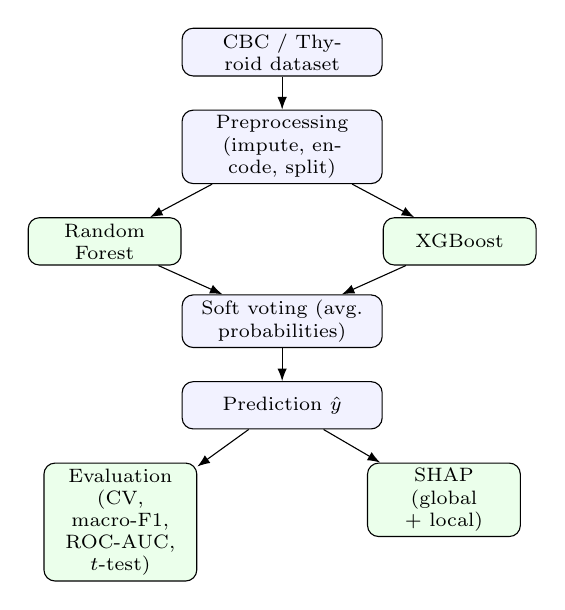
\begin{tikzpicture}[
  node distance=4.2mm and 6mm,
  box/.style={draw, rounded corners, align=center, font=\scriptsize,
              minimum height=6mm, inner sep=2pt, fill=blue!5, text width=24mm},
  base/.style={draw, rounded corners, align=center, font=\scriptsize,
              minimum height=6mm, inner sep=2pt, fill=green!8, text width=18mm},
  arr/.style={-{Latex[length=1.6mm]}}]
\node[box] (data) {CBC / Thyroid dataset};
\node[box, below=of data] (prep) {Preprocessing\\(impute, encode, split)};
\node[base, below left=of prep, xshift=6mm] (rf) {Random Forest};
\node[base, below right=of prep, xshift=-6mm] (xgb) {XGBoost};
\node[box, below=14mm of prep] (vote) {Soft voting (avg.\ probabilities)};
\node[box, below=of vote] (pred) {Prediction $\hat{y}$};
\node[base, below left=of pred, xshift=8mm] (eval) {Evaluation\\(CV, macro-F1,\\ROC-AUC, $t$-test)};
\node[base, below right=of pred, xshift=-8mm] (shap) {SHAP\\(global + local)};
\draw[arr] (data) -- (prep);
\draw[arr] (prep) -- (rf);
\draw[arr] (prep) -- (xgb);
\draw[arr] (rf) -- (vote);
\draw[arr] (xgb) -- (vote);
\draw[arr] (vote) -- (pred);
\draw[arr] (pred) -- (eval);
\draw[arr] (pred) -- (shap);
\end{tikzpicture}
\caption{The shared, leakage-safe pipeline used for both experiments.}
\label{fig:arch}
\end{figure}

\section{Results}
\subsection{Experiment 1: Anemia}
Table~\ref{tab:anemia_cv} reports five-fold cross-validation. The hybrid attains
$0.987$ accuracy and $0.939$ macro-F1. On the hold-out test set the hybrid attains
accuracy $0.984$, macro-F1 $0.947$, and ROC--AUC $0.9997$ (Table~\ref{tab:test}).
Per-class F1 exceeds $0.94$ for all well-populated classes; the sole weak class is
Macrocytic anemia (F1 $0.67$ on three test samples), a small-sample artifact.
Notably, the \emph{stacking} extension achieves the best cross-validated macro-F1
($0.966$), the one configuration that clearly surpasses the soft-voting hybrid.

The paired $t$-test of hybrid versus RF yields $\bar{d}{=}{+}0.0053$,
$t{=}0.24$, $p{=}0.82$: \emph{not} significant. On roughly $1{,}200$ patients the
hybrid's edge over a strong baseline is within fold noise.

\begin{table}[t]
\caption{Experiment 1 (Anemia): stratified five-fold cross-validation,
mean\,$\pm$\,std.}
\label{tab:anemia_cv}
\centering
\renewcommand{\arraystretch}{1.2}
\begin{tabular}{lccc}
\toprule
\textbf{Model} & \textbf{Accuracy} & \textbf{Macro-F1} & \textbf{ROC-AUC} \\
\midrule
Random Forest        & $0.985\pm0.013$ & $0.934\pm0.055$ & $0.9996$ \\
XGBoost              & $0.988\pm0.004$ & $0.948\pm0.008$ & $0.9994$ \\
Hybrid (RF$+$XGB)    & $0.987\pm0.007$ & $0.939\pm0.017$ & $0.9998$ \\
LightGBM             & $0.989\pm0.006$ & $0.947\pm0.053$ & $0.9997$ \\
Stacking             & $\mathbf{0.991\pm0.006}$ & $\mathbf{0.966\pm0.025}$ & $0.9998$ \\
\bottomrule
\end{tabular}
\end{table}

\begin{figure}[t]
\centering
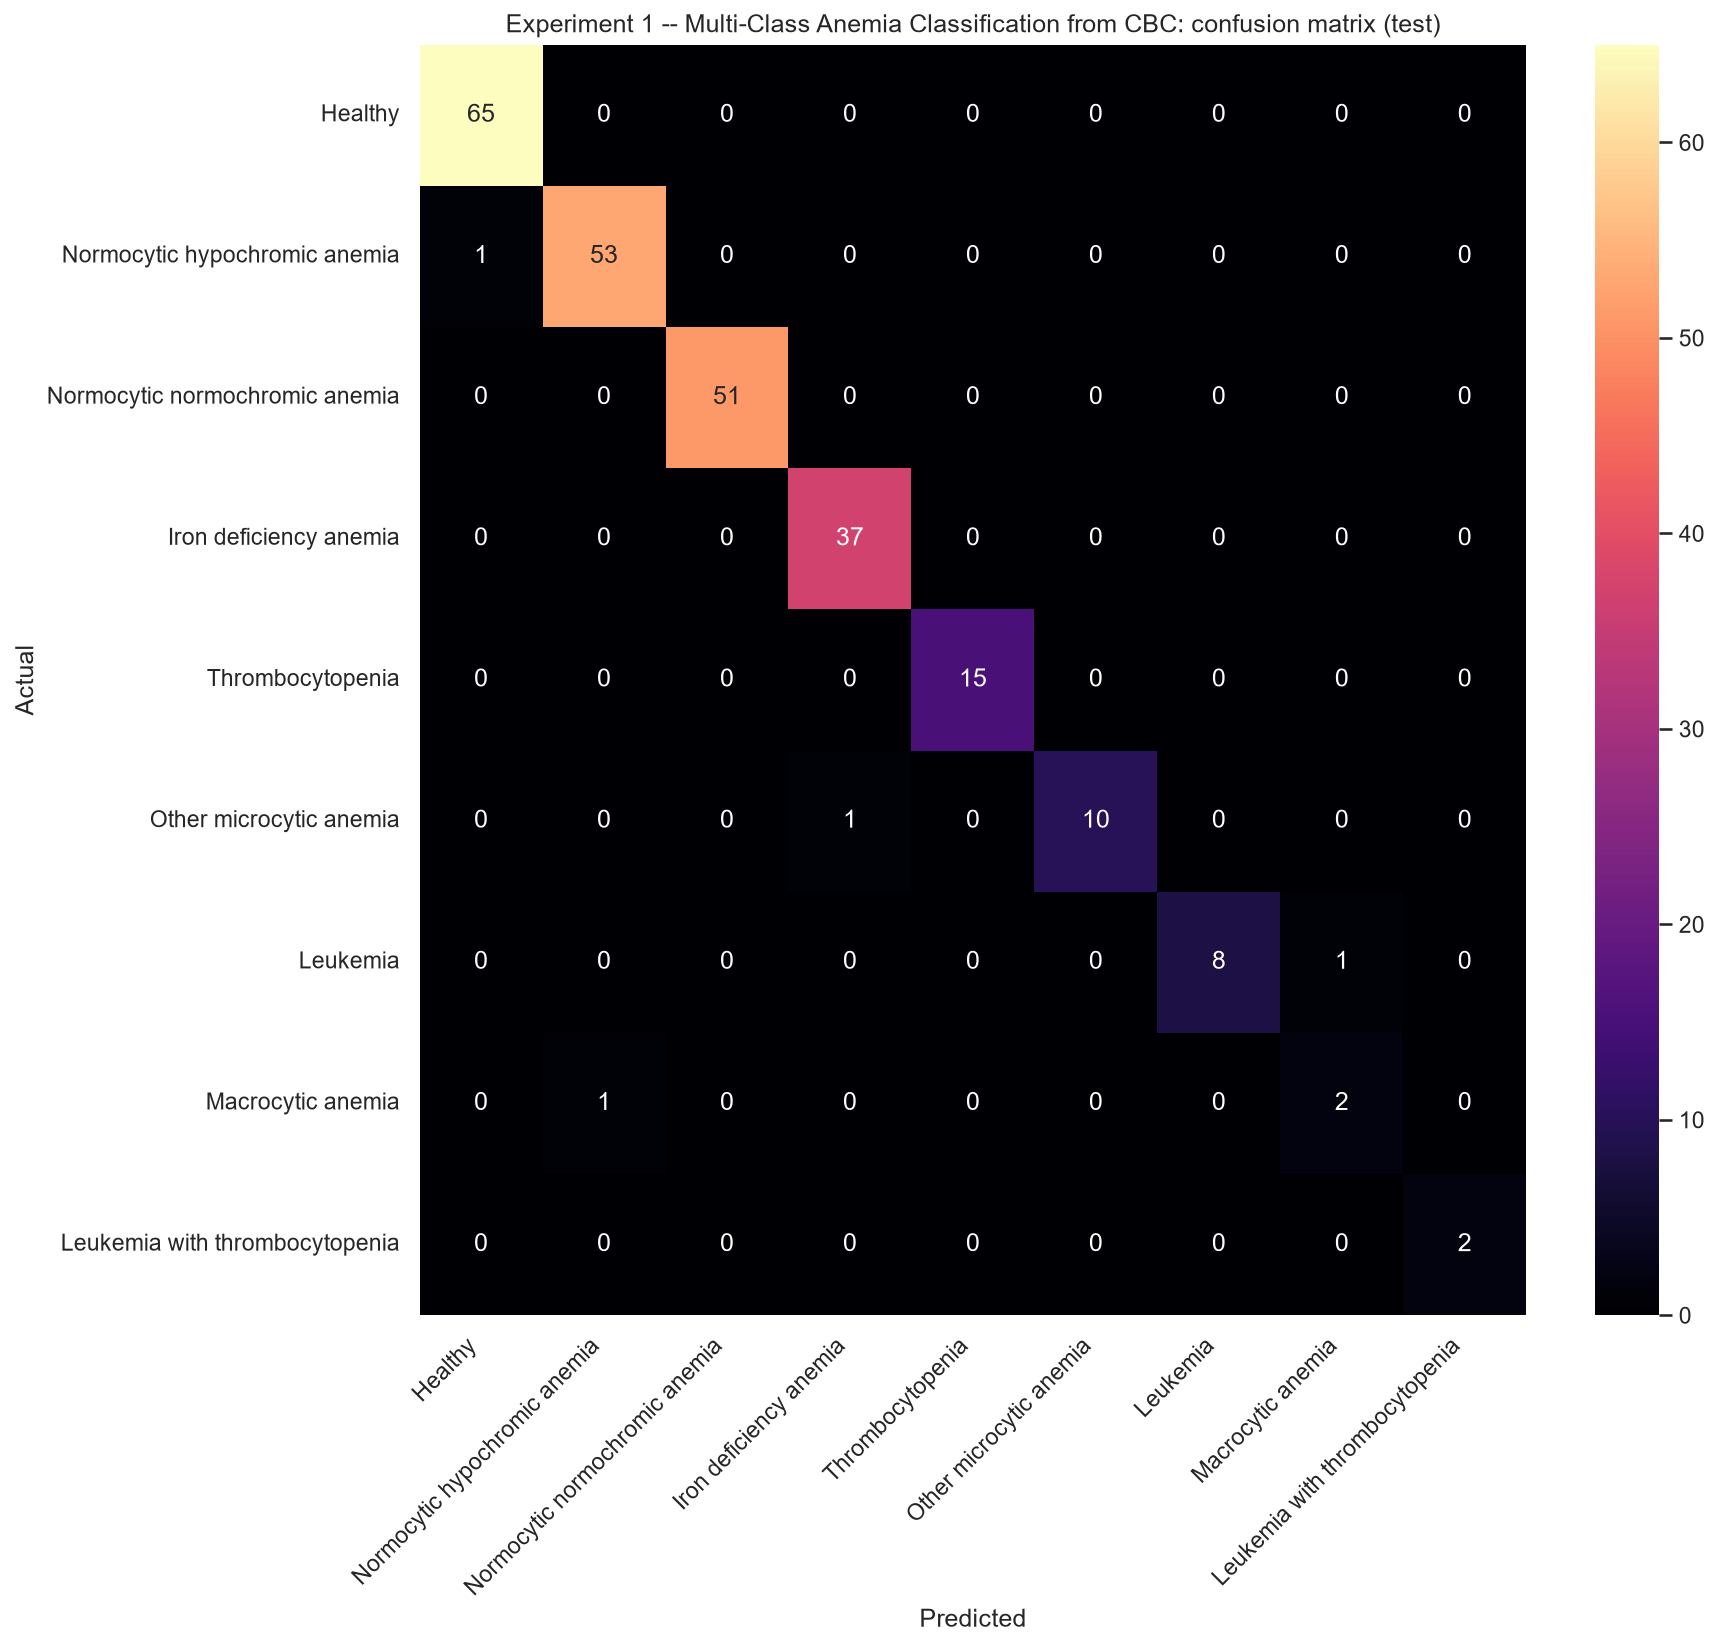
\includegraphics[width=0.92\columnwidth]{anemia_cm.png}
\caption{Experiment 1: confusion matrix of the hybrid on the anemia hold-out set.}
\label{fig:anemia_cm}
\end{figure}

\subsection{Experiment 2: Thyroid (Extension)}
Table~\ref{tab:thyroid_cv} reports cross-validation on the thyroid data. The
hybrid attains $0.952$ accuracy and $0.875$ macro-F1; on the hold-out set it
attains accuracy $0.945$, balanced accuracy $0.850$, macro-F1 $0.863$, and
ROC--AUC $0.995$ (Table~\ref{tab:test}). The gap between accuracy ($0.945$) and
macro-F1 ($0.863$) is the imbalance story in one line: the model is excellent on
large classes and merely good on rare ones. Per-class results
(Table~\ref{tab:thyroid_pc}) show near-perfect detection of hypothyroidism
(F1~$0.967$) but difficulty on the intrinsically ambiguous discordant-results
class (F1~$0.633$)---a class defined by \emph{disagreeing} assays, where no clean
signal exists.

Here the paired $t$-test of hybrid versus RF yields $\bar{d}{=}{+}0.0255$,
$t{=}4.16$, $p{=}0.014$: \emph{significant}. The same kind of improvement that was
undetectable on $1{,}200$ anemia patients becomes detectable on $9{,}172$ thyroid
patients---a direct illustration of statistical power.

\begin{table}[t]
\caption{Experiment 2 (Thyroid): stratified five-fold cross-validation,
mean\,$\pm$\,std.}
\label{tab:thyroid_cv}
\centering
\renewcommand{\arraystretch}{1.2}
\begin{tabular}{lccc}
\toprule
\textbf{Model} & \textbf{Accuracy} & \textbf{Macro-F1} & \textbf{ROC-AUC} \\
\midrule
Random Forest        & $0.941\pm0.008$ & $0.850\pm0.024$ & $0.992$ \\
XGBoost              & $0.950\pm0.006$ & $0.872\pm0.020$ & $0.995$ \\
Hybrid (RF$+$XGB)    & $\mathbf{0.952\pm0.005}$ & $\mathbf{0.875\pm0.018}$ & $0.995$ \\
LightGBM             & $0.951\pm0.005$ & $0.873\pm0.018$ & $0.994$ \\
Stacking             & $0.951\pm0.005$ & $0.874\pm0.015$ & $0.991$ \\
\bottomrule
\end{tabular}
\end{table}

\begin{table}[t]
\caption{Experiment 2 (Thyroid): per-class hold-out performance of the hybrid.}
\label{tab:thyroid_pc}
\centering
\renewcommand{\arraystretch}{1.2}
\begin{tabular}{lcccc}
\toprule
\textbf{Class} & \textbf{Prec.} & \textbf{Rec.} & \textbf{F1} & \textbf{Support} \\
\midrule
negative              & 0.963 & 0.974 & 0.969 & 1355 \\
hypothyroid           & 0.949 & 0.985 & 0.967 & 132 \\
nonthyroidal illness  & 0.977 & 0.923 & 0.949 & 91 \\
binding protein       & 0.829 & 0.808 & 0.818 & 78 \\
replacement therapy   & 0.903 & 0.915 & 0.909 & 71 \\
discordant results    & 0.738 & 0.554 & 0.633 & 56 \\
hyperthyroid          & 0.804 & 0.789 & 0.796 & 52 \\
\midrule
macro avg             & 0.880 & 0.850 & 0.863 & 1835 \\
\bottomrule
\end{tabular}
\end{table}

\begin{table}[t]
\caption{Hold-out test performance of the hybrid in both experiments.}
\label{tab:test}
\centering
\renewcommand{\arraystretch}{1.2}
\begin{tabular}{lcc}
\toprule
\textbf{Metric} & \textbf{Anemia} & \textbf{Thyroid} \\
\midrule
Accuracy          & 0.984 & 0.945 \\
Balanced accuracy & 0.939 & 0.850 \\
Macro-F1          & 0.947 & 0.863 \\
Weighted-F1       & 0.984 & 0.944 \\
ROC--AUC (OvR)    & 0.9997 & 0.995 \\
\bottomrule
\end{tabular}
\end{table}

\subsection{p-Value Stability}
\label{sec:stability}
Because $n{=}5$, the paired $t$-test is high-variance. Holding the data and models
fixed and varying only the fold-shuffling seed, the hybrid-versus-RF p-value on
anemia ranges from $0.03$ to $0.99$ (Table~\ref{tab:pstab}); nine of ten seeds are
non-significant, one crosses $0.05$ by chance. Our $0.82$ is an unremarkable draw
from this distribution. The robust outcome is therefore the \emph{verdict} (not
significant), not any single p-value---a caution against over-interpreting one
statistic from few folds.

\begin{table}[t]
\caption{Anemia hybrid-vs-RF paired $t$-test under different fold seeds.}
\label{tab:pstab}
\centering
\renewcommand{\arraystretch}{1.15}
\begin{tabular}{cccc}
\toprule
\textbf{Seed} & \textbf{mean(Hyb$-$RF)} & \textbf{p-value} & \textbf{Verdict} \\
\midrule
13   & $+0.0002$ & 0.990 & not sig. \\
42   & $+0.0053$ & 0.824 & not sig. \\
0    & $+0.0067$ & 0.762 & not sig. \\
21   & $+0.0184$ & 0.425 & not sig. \\
7    & $+0.0204$ & 0.118 & not sig. \\
99   & $+0.0325$ & \textbf{0.029} & \textbf{significant} \\
\midrule
\multicolumn{4}{l}{\footnotesize Range over 10 seeds: $[0.029,\,0.990]$;
significant in $10\%$.} \\
\bottomrule
\end{tabular}
\end{table}

\section{Explainability Analysis}
\subsection{Global Attribution}
For anemia, the top global SHAP features are HGB, MCV, WBC, MCHC, MCH, and PLT,
recovering the MCV-centered morphological framework that underpins hematologic
diagnosis. For thyroid, the top features are
TSH, T3, FTI, TT4, on-thyroxine, and T4U---exactly the thyroid function panel,
ordered as a clinician would expect (Fig.~\ref{fig:thy_shap}). The
missing-indicator features for T3 and TSH also rank highly, confirming that
\emph{which} tests were ordered carries diagnostic signal.

\begin{figure}[t]
\centering
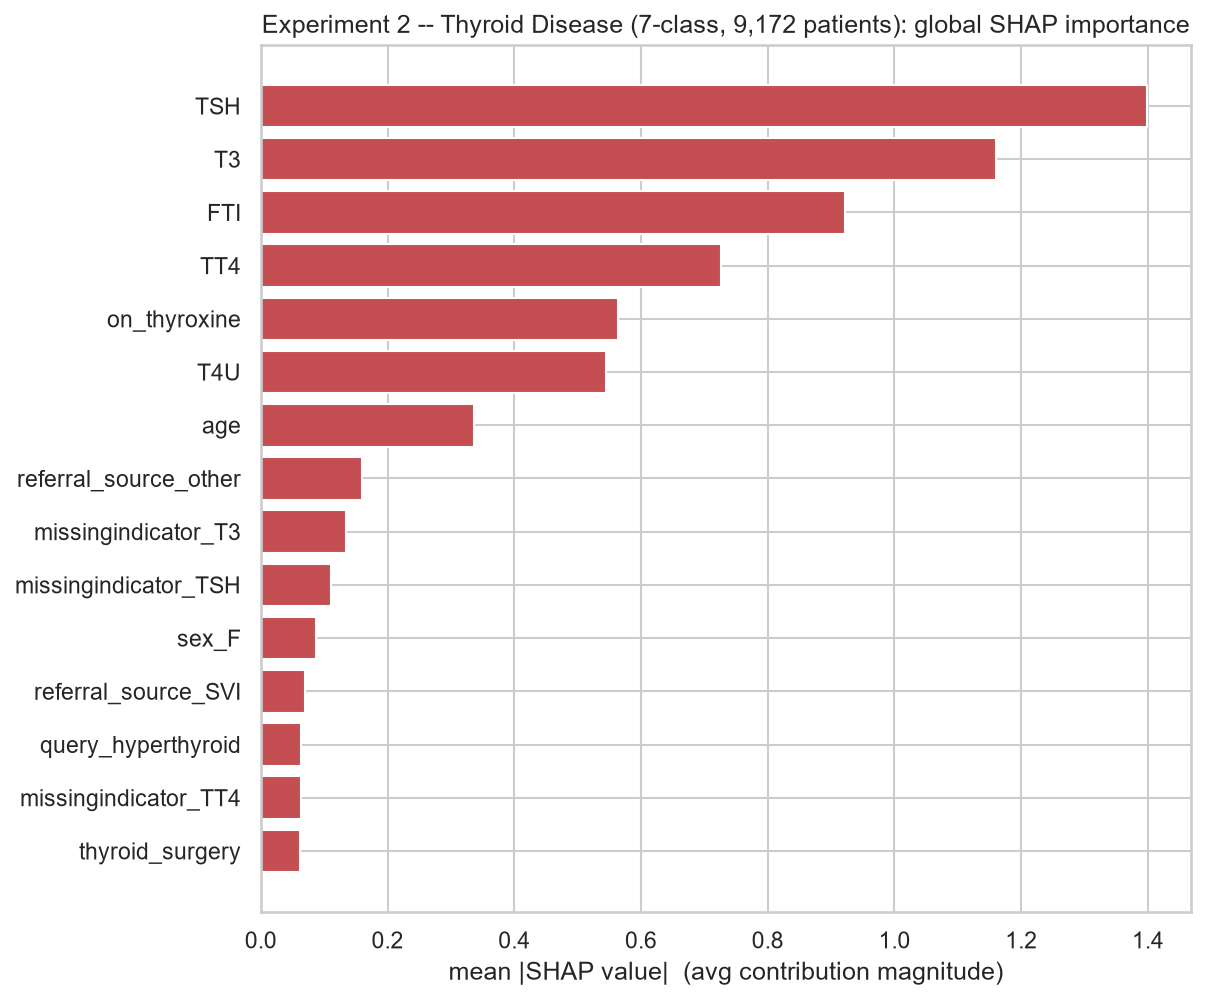
\includegraphics[width=0.95\columnwidth]{thyroid_shap_bar.png}
\caption{Experiment 2: global SHAP importance (mean $|\phi_j|$) of the XGBoost
component on the thyroid data.}
\label{fig:thy_shap}
\end{figure}

\subsection{Per-Prediction Explanation}
Equation~(\ref{eq:shap}) lets us narrate individual predictions. For a thyroid
patient predicted \textit{hyperthyroid} (Fig.~\ref{fig:thy_wf}), the dominant
contributions are a very high free thyroxine index (FTI$\,{=}\,196$) and a
suppressed TSH ($0.02$)---the textbook signature of an overactive gland under
negative feedback. For an anemia patient predicted \textit{iron deficiency}, low
MCV and low MCH drive the decision, matching the microcytic--hypochromic
phenotype. Because contributions sum to the model output, each explanation is a
complete account rather than a post-hoc rationalization.

\begin{figure}[t]
\centering
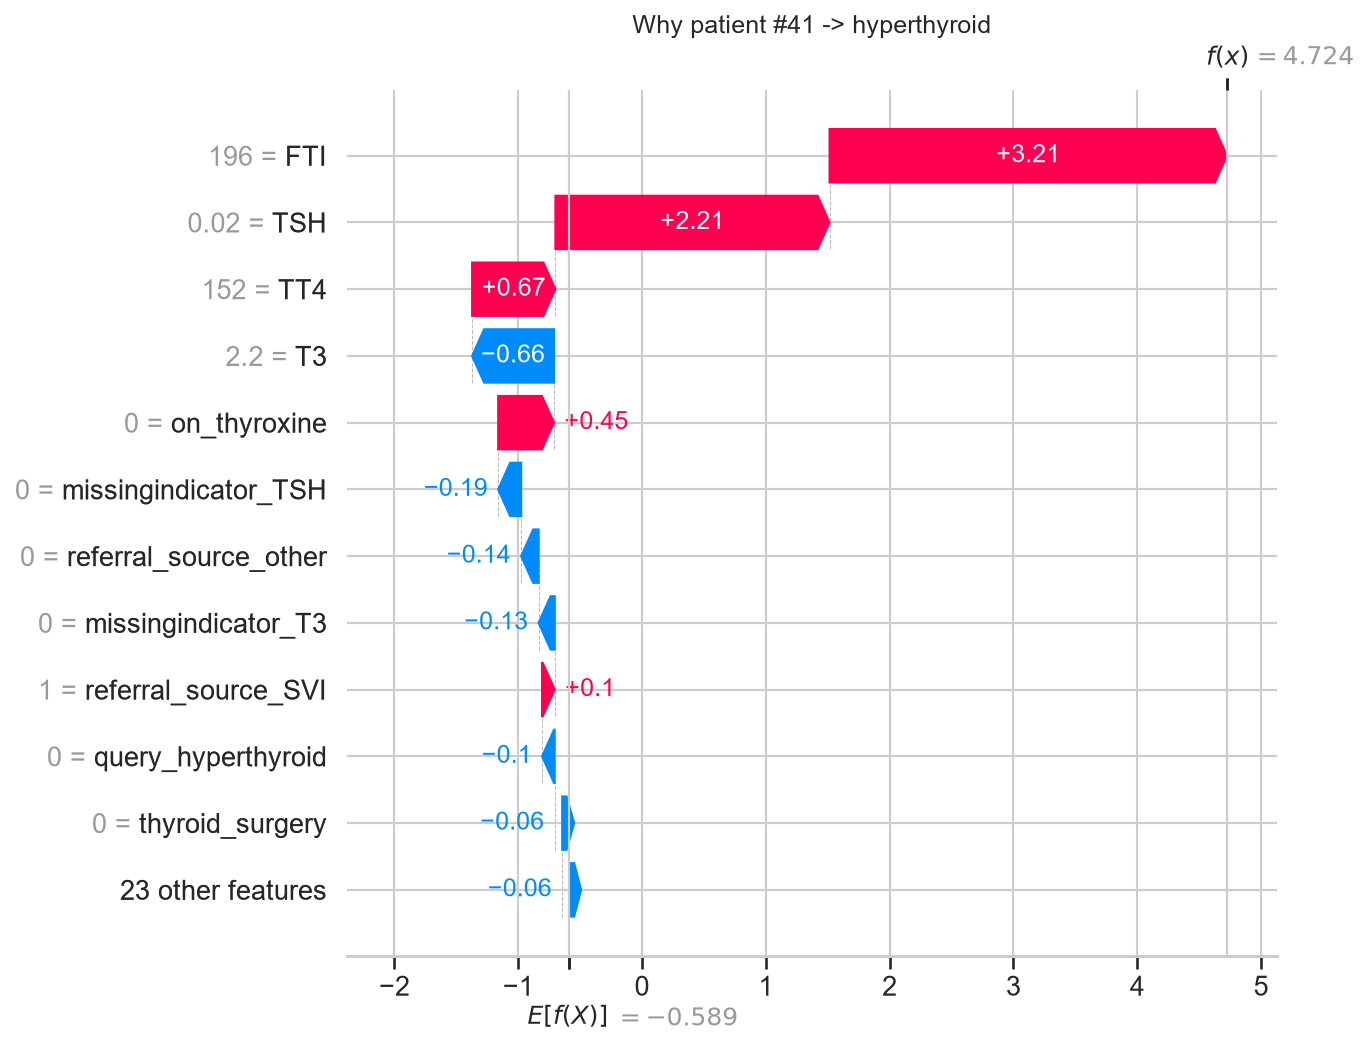
\includegraphics[width=0.97\columnwidth]{thyroid_waterfall_hyper.png}
\caption{Experiment 2: per-prediction SHAP waterfall for a patient correctly
predicted as hyperthyroid; FTI and suppressed TSH dominate.}
\label{fig:thy_wf}
\end{figure}

\subsection{Explaining Errors and Data Quality}
SHAP applied to mis-classified cases is diagnostically useful. One anemia patient
labeled \textit{Normocytic hypochromic} but predicted \textit{Healthy} carries
physiologically impossible values (HGB$\,{=}\,41$, RBC$\,{=}\,13.1$,
HCT$\,{=}\,2$); the SHAP decomposition shows the absurd HGB drove the error,
turning a silent misclassification into a visible, diagnosable data-quality
problem. This exemplifies interpretability as a debugging tool, not merely a
trust signal.

\section{Discussion}
Three findings stand out. First, the anemia results are strong and stable,
including an honest negative significance result. Second, scaling to a $7\times$
larger, imbalanced, missingness-laden
thyroid problem is feasible with the same pipeline, but the macro-F1 drops to
$0.863$---not because the model is worse, but because the problem is harder and the
evaluation is more honest (an intrinsically ambiguous class and severe imbalance).
Third, the significance contrast ($p{=}0.82$ on anemia versus $p{=}0.014$ on
thyroid), together with the seed-stability analysis, makes a methodological point
that transcends either dataset: with few folds and a near-zero effect, a p-value is
noise, and only sample size makes a small true effect detectable. Throughout,
SHAP explanations agree with physiology and occasionally reveal data problems,
supporting their inclusion in clinical decision-support pipelines.

\section{Limitations}
Both datasets are single-institution and, for thyroid, decades old; external
multi-center validation is needed. The thyroid class grouping is a modeling choice
that merges fine-grained diagnoses. Hyperparameters were only lightly tuned, and
SHAP provides associational, not causal, attributions. Minority classes
(Macrocytic anemia; discordant thyroid results) remain under-represented, limiting
the reliability of their per-class estimates.

\section{Conclusion}
We presented a reproducible, explainable hybrid ML framework and validated it on
two multi-class disease problems. Experiment~1 is a nine-class anemia classifier
with an honest non-significant model comparison. Experiment~2 extends the pipeline
to a larger, harder seven-class thyroid problem,
explicitly handling imbalance and informative missingness, and shows that the
hybrid's advantage becomes statistically significant only with more data. Detailed
per-prediction SHAP explanations align with established physiology and can surface
data-quality errors. Future work includes external validation, cost-sensitive
learning for rare classes, SHAP interaction analysis, and probability calibration
for clinically actionable confidence estimates.

\begin{thebibliography}{1}
\bibitem{ref_rf}
L.~Breiman, ``Random Forests,'' \emph{Machine Learning}, vol.~45, no.~1,
pp.~5--32, 2001.
\bibitem{ref_xgb}
T.~Chen and C.~Guestrin, ``XGBoost: A Scalable Tree Boosting System,'' in
\emph{Proc.\ ACM SIGKDD}, 2016, pp.~785--794.
\bibitem{ref_shap}
S.~M. Lundberg and S.-I. Lee, ``A Unified Approach to Interpreting Model
Predictions,'' in \emph{Adv.\ Neural Inf.\ Process.\ Syst.\ (NeurIPS)}, 2017.
\bibitem{ref_treeshap}
S.~M. Lundberg \emph{et al.}, ``From Local Explanations to Global Understanding
with Explainable AI for Trees,'' \emph{Nat.\ Mach.\ Intell.}, vol.~2, pp.~56--67,
2020.
\bibitem{ref_garavan}
J.~R. Quinlan \emph{et al.}, ``Thyroid Disease Records,'' Garavan Institute, UCI
Machine Learning Repository, 1987.
\bibitem{ref_lightgbm}
G.~Ke \emph{et al.}, ``LightGBM: A Highly Efficient Gradient Boosting Decision
Tree,'' in \emph{NeurIPS}, 2017.
\end{thebibliography}

\end{document}
